\documentclass[12pt]{scrartcl}
 \usepackage{fancyhdr, graphicx}
 \usepackage[german]{babel}
 \usepackage[scaled=0.92]{helvet}
 \usepackage{enumitem}
 \usepackage{parskip}
 \usepackage{lastpage} % for getting last page number
\usepackage{listings}
\usepackage{caption}
\usepackage{color}
\usepackage{xcolor}
\DeclareCaptionFont{white}{\color{white}}
\DeclareCaptionFormat{listing}{\colorbox{gray}{\parbox{\textwidth}{#1#2#3}}}
\captionsetup[lstlisting]{format=listing,labelfont=white,textfont=white}
\lstset{
 language=Java,
 basicstyle=\footnotesize\ttfamily, % Standardschrift
 numbers=left,               % Ort der Zeilennummern
 numberstyle=\tiny,          % Stil der Zeilennummern
 stepnumber=5,              % Abstand zwischen den Zeilennummern
 numbersep=5pt,              % Abstand der Nummern zum Text
 tabsize=2,                  % Groesse von Tabs
 extendedchars=true,         %
 breaklines=true,            % Zeilen werden Umgebrochen
 frame=b,         
 %commentstyle=\itshape\color{LightLime}, Was isch das? O_o
 %keywordstyle=\bfseries\color{DarkPurple}, und das O_o
 basicstyle=\small,
 stringstyle=\color[RGB]{42,0,255}\ttfamily, % Farbe der String
 keywordstyle=\color[RGB]{127,0,85}\ttfamily, % Farbe der Keywords
 commentstyle=\color[RGB]{63,127,95}\ttfamily, % Farbe des Kommentars
 showspaces=false,           % Leerzeichen anzeigen ?
 showtabs=false,             % Tabs anzeigen ?
 xleftmargin=17pt,
 framexleftmargin=17pt,
 framexrightmargin=5pt,
 framexbottommargin=4pt,
 showstringspaces=false      % Leerzeichen in Strings anzeigen ?        
}
\newcommand\Fontvi{\fontsize{6}{7.2}\selectfont}

 \renewcommand{\familydefault}{\sfdefault}
 
 \fancypagestyle{firststyle}{ %Style of the first page
 \fancyhf{}
 \fancyheadoffset[L]{0.6cm}
 \lhead{
 
\includegraphics[scale=0.8]{./fhnw_ht_e_10mm.jpg}}
 \renewcommand{\headrulewidth}{0pt}
 \lfoot{APSI Lab 1}
 \rfoot{Roland Hediger, Jonas Schwammberger}
}

\fancypagestyle{documentstyle}{ %Style of the rest of the document
 \fancyhf{}
 \fancyheadoffset[L]{0.6cm}
\lhead{
 
\includegraphics[scale=0.8]{./fhnw_ht_e_10mm.jpg}}
 \renewcommand{\headrulewidth}{0pt}
 \lfoot{\thepage\ / \pageref{LastPage} }
}

\pagestyle{firststyle} %different look of first page
 
\title{ %Titel
APSI Lab 1
\vspace{0.2cm}
}

 \begin{document}
 \maketitle
 \thispagestyle{firststyle}
 \pagestyle{firststyle}
 \begin{abstract}
 \begin{center}
  put abstract here  
 \end{center}
 \vspace{0.5cm}
\hrulefill
\end{abstract}

 \pagestyle{documentstyle}
 \tableofcontents
 \pagebreak
\section{Aufgabenstellung}
Ihre Aufgabe besteht darin, sogenannte Kollisionen im Hash-Verfahren zu suchen, d.h. Änderungen
im Originaltext, die den gleichen Hashwert liefern: $ h(m_{orig}) = h(m_{fake})$. Wie Sie vielleicht
bereits bemerkt haben, handelt es sich um eine praktische Anwendung des bekannten
Geburtstagsparadoxons, das Sie in der Mathematik bzw. in der Kryptologie kennengelernt
haben.

\section{Softwareaufbau}
Die Aufgabe wurde mit zwei Klassen implementiert. Die Klasse \"SimplifiedHash\" beinhaltet die beschriebene Hashfunktion und in der Klasse \"CollisionGenerator\" werden die verschiedenen Kombinationen der Mails generiert und nach einer Hashkollision überprüft.

\subsection{Hashfunktion}
Die Hashfunktion wurde nach der Spezifikation der Aufgabenstellung implementiert. Jedoch hat der DES Cipher eine Output-Länge von  128 Bit, wie man die 128 Bit verkürzen soll auf 64 Bit ist nicht spezifiziert. Deshalb wird der DES-Output in zwei 64-Bit-Blöcke aufgeteilt und mit XOR auf einen 64-Bit-Block eingestampft.

\subsection{Kollisionsgenerator}
\subsubsection{Variationserzeugung}
Lauf der Aufgabenstellung haben wir $2^{32}$ verschiedene Kombinationsmöglichkeiten pro Mail. Diese Kombinationen haben wir in einem Integer codiert, dabei repräsentiert ein Bit einen Platzhalter.   Zum Beispiel: Das zweite Bit steht auf 0, dann wird das Wort "vom Herzen" eingesetzt. So können wir jede Variation eindeutig bestimmen.
Es lohnt sich nicht, nach jeder neu generierten Variation (je von einem Original-Mail und einem Fake-Mail) nach einer Kollision zu suchen, werden immer 1024 Variationen generiert und nachher nach Kollisionen gesucht.

\subsection{Kollisionsdetektion}
\subsubsection{Strategien}
Wir können zwischen zwei Strateien unterscheiden. Entweder, wir generieren alle Original und Fake Variationen linear (beginnend bei 0), oder wir je einen Random Integer für die Original und die Fake Mail. Mit der Random Strategie erhoffen wir uns eine bessere Laufzeit und kleineren Memory Footprint falls man nach mehreren Kollisionen sucht.

\subsubsection{Datenstrukturen}
Wir haben zwei Hashmaps, eine für alle Variationen der Original-Mail und eine für die Fake-Mail. Für den Key benutzen wir jeweils den Hashwert und als Value wird der Variations-Integer dieser Mail gesetzt. So können wir bei der Kollisionsdetektion durch die Schlüssel der Original-Mail-Hashmap

\section{Anhang}
\begin{lstlisting}
package ch.fhnw.apsi.lab1;

import java.nio.ByteBuffer;
import java.nio.ByteOrder;

import org.bouncycastle.crypto.BlockCipher;
import org.bouncycastle.crypto.BufferedBlockCipher;
import org.bouncycastle.crypto.CryptoException;
import org.bouncycastle.crypto.engines.DESEngine;
import org.bouncycastle.crypto.modes.PaddedBlockCipher;
import org.bouncycastle.crypto.params.KeyParameter;

public class SimplifiedHash {
	private final static byte[] iv = { (byte) 0b10101010, (byte) 0b10101010, (byte) 0b10101010, (byte) 0b10101010, (byte) 0b10101010, (byte) 0b10101010, (byte) 0b10101010,
			(byte) 0b10101010 };

	private byte[] preprocess(byte[] input) {
		int mLength = input.length;
		byte[] length = ByteBuffer.allocate(8).putLong(mLength).array();
		int r = 8 - mLength % 8; // calculate the rest you need to make the
									// input divisible by 8
		byte[] out = new byte[mLength + r + 8];

		// Copy
		for (int i = 0; i < mLength; i++)
			out[i] = input[i];
		// padding
		if (r > 0)
			out[mLength] = -128; // 0b1000 0000

		for (int i = 1; i < r; i++)
			out[mLength + i] = 0;

		// add message length
		for (int i = 0; i < 8; i++)
			out[out.length - 8 + i] = length[i];

		return out;
	}

	private long create(byte[] input) {
		BlockCipher engine = new DESEngine();
		@SuppressWarnings("deprecation")
		BufferedBlockCipher cipher = new PaddedBlockCipher(engine);
		byte[] desOut = new byte[16];
		byte[] hash = new byte[8];
		byte[] previousHash = iv.clone();

		for (int i = 0; i < input.length; i += 8) {
			KeyParameter p = new KeyParameter(previousHash);
			cipher.init(true, p);
			desOut = new byte[cipher.getOutputSize(8)];
			int outputLen = cipher.processBytes(input, i, 8, desOut, 0);

			try {
				cipher.doFinal(desOut, 0);

				// xor magix
				for (int j = 0; j < hash.length; j++)
					hash[j] = (byte) (desOut[j] ^ desOut[j + 8] ^ previousHash[j]);

				// swap
				byte[] tmp = hash;
				hash = previousHash;
				previousHash = tmp;

			} catch (CryptoException ce) {
				System.err.println(ce);
			}

		}

		ByteBuffer buffer = ByteBuffer.wrap(previousHash);
		buffer.order(ByteOrder.LITTLE_ENDIAN);
		return buffer.getLong();
	}

	public int createHash(byte[] input) {
		long hash = this.create(this.preprocess(input));
		int h1 = (int) (hash >>> 32);
		int h2 = Integer.reverse((int) hash);

		return h1 ^ h2;
	}

}

\end{lstlisting}

\begin{figure} [h!]

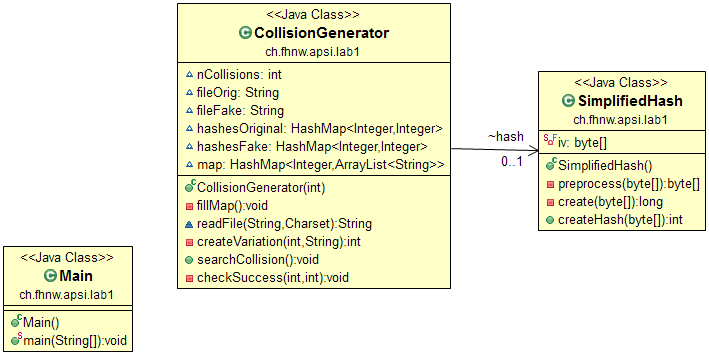
\includegraphics[scale= 0.5]{apsi_lab.png}
\caption{Klassendiagramm}
\end{figure}

 \end{document}